\documentclass{article}

% if you need to pass options to natbib, use, e.g.:
%     \PassOptionsToPackage{numbers, compress}{natbib}
% before loading neurips_2026
\PassOptionsToPackage{numbers, compress}{natbib}

% The authors should use one of these tracks.
% Before accepting by the NeurIPS conference, select one of the options below.
% 0. "default" for submission
\usepackage{neurips_2026}
% the "default" option is equal to the "main" option, which is used for the Main Track with double-blind reviewing.
% 1. "main" option is used for the Main Track
%  \usepackage[main]{neurips_2026}
% 2. "position" option is used for the Position Paper Track
%  \usepackage[position]{neurips_2026}
% 3. "eandd" option is used for the Evaluations & Datasets Track
 % \usepackage[eandd]{neurips_2026}
 % if you want to opt-in for a de-anomymized submission (not recommended, but OK):
 %\usepackage[eandd, nonanonymous]{neurips_2026}
% 4. "creativeai" option is used for the Creative AI Track
%  \usepackage[creativeai]{neurips_2026}
% 5. "sglblindworkshop" option is used for the Workshop with single-blind reviewing
 % \usepackage[sglblindworkshop]{neurips_2026}
% 6. "dblblindworkshop" option is used for the Workshop with double-blind reviewing
%  \usepackage[dblblindworkshop]{neurips_2026}

% After being accepted, the authors should add "final" behind the track to compile a camera-ready version.
% 1. Main Track
 % \usepackage[main, final]{neurips_2026}
% 2. Position Paper Track
%  \usepackage[position, final]{neurips_2026}
% 3. Evaluations & Datasets Track
 % \usepackage[eandd, final]{neurips_2026}
% 4. Creative AI Track
%  \usepackage[creativeai, final]{neurips_2026}
% 5. Workshop with single-blind reviewing
%  \usepackage[sglblindworkshop, final]{neurips_2026}
% 6. Workshop with double-blind reviewing
%  \usepackage[dblblindworkshop, final]{neurips_2026}
% Note. For the workshop paper template, both \title{} and \workshoptitle{} are required, with the former indicating the paper title shown in the title and the latter indicating the workshop title displayed in the footnote.
% For workshops (5., 6.), the authors should add the name of the workshop, "\workshoptitle" command is used to set the workshop title.
% \workshoptitle{WORKSHOP TITLE}

% "preprint" option is used for arXiv or other preprint submissions
 % \usepackage[preprint]{neurips_2026}

% to avoid loading the natbib package, add option nonatbib:
%    \usepackage[nonatbib]{neurips_2026}

\usepackage[utf8]{inputenc} % allow utf-8 input
\usepackage[T1]{fontenc}    % use 8-bit T1 fonts
\usepackage{hyperref}       % hyperlinks
\usepackage{url}            % simple URL typesetting
\usepackage{booktabs}       % professional-quality tables
\usepackage{multirow}       % multi-row table cells
\usepackage{amsmath}        % math environments and \text{}
\usepackage{amsfonts}       % blackboard math symbols
\usepackage{amssymb}        % extra math symbols
\usepackage{nicefrac}       % compact symbols for 1/2, etc.
\usepackage{microtype}      % microtypography
\usepackage{xcolor}         % colors
\usepackage{pifont}
\usepackage{graphicx}
% Note. For the workshop paper template, both \title{} and \workshoptitle{} are required, with the former indicating the paper title shown in the title and the latter indicating the workshop title displayed in the footnote.
\title{TinyVLM: Temporal Token Reuse and Adaptive Routing for Efficient Edge Vision-Language Models}


% The \author macro works with any number of authors. There are two commands
% used to separate the names and addresses of multiple authors: \And and \AND.
%
% Using \And between authors leaves it to LaTeX to determine where to break the
% lines. Using \AND forces a line break at that point. So, if LaTeX puts 3 of 4
% authors names on the first line, and the last on the second line, try using
% \AND instead of \And before the third author name.


\author{%
  Anonymous Submission \\
  Paper under double-blind review \\
}


\begin{document}


\maketitle


\begin{abstract}
Deploying vision-language models (VLMs) on edge devices remains challenging due to strict constraints on computation, memory, and energy. We propose a unified compression framework that exploits spatio-temporal redundancy and input-adaptive computation to enable efficient multimodal reasoning. Our approach introduces Sparse Temporal Token Fusion (STTF), which reduces redundant visual tokens by selectively updating regions of change across time, and Adaptive Neural Compression (ANC), which dynamically scales model capacity via input-conditioned encoder routing. A Switch-Transformer-style load-balancing loss ensures ANC routing remains genuinely adaptive across all branches, preventing collapse to a single path. Built on a frozen CLIP ViT-B/32 visual encoder with three lightweight ANC projection heads and a transformer caption decoder, our system achieves CIDEr~$\mathbf{82.69 \pm 0.84}$ and BLEU-4~$\mathbf{26.12 \pm 0.18}$ on MS-COCO captioning over three matched seeds (15 epochs; a 50-epoch single-seed run reaches CIDEr~$89.72$) at $\sim$17.6~GFLOPs per inference (hard-routing average). On the same three seeds, this is a \textbf{$+30.30$~CIDEr improvement over a matched-seed TokenLearner baseline} ($52.39 \pm 3.39$; paired $t_{2}{=}{+}24.79$, $p{=}0.002$, Cohen's $d{=}{+}11.90$, 95\%~CI $[{+}27.38,\,{+}32.03]$), at comparable inference cost. To validate the routing and STTF mechanics in isolation we additionally train a 21M-parameter scratch CNN backbone over the same three seeds, achieving CIDEr~$36.70 \pm 0.37$ at $\sim$10.3~GFLOPs; this CNN proof-of-concept trades CIDEr for FLOPs ($-15.7$~CIDEr vs.\ TokenLearner, paired $t_{2}{=}{-}7.40$, $p{=}0.018$, $d{=}{-}4.27$) but reproduces the routing behaviour the full system relies on. Routing utilization stays balanced ($31\%$/$34\%$/$35\%$) across training; a cross-$\tau$ sweep ($\tau \in [0.70, 0.90]$) varies CIDEr by only $0.45$ points; on event streams, STTF cuts FLOPs by $83\%$ on N-Caltech101 with negligible accuracy loss. Together these results demonstrate that structured, input-aware compression --- when paired with a strong pretrained visual backbone --- yields competitive captioning quality at edge-deployable cost.
\end{abstract}



\section{Introduction}
Vision-language models (VLMs) have rapidly advanced the state of the art in multimodal reasoning, enabling strong performance across tasks such as image captioning, visual question answering, and embodied perception. These gains have largely been driven by scaling model size and compute, following trends established in large language models and vision transformers. However, this scaling paradigm presents a fundamental challenge: modern VLMs are prohibitively expensive to deploy in resource-constrained environments, including mobile devices, drones, and embedded systems, where strict limits on latency, memory, and energy consumption must be satisfied.

A growing body of work has explored model compression techniques such as pruning, quantization, and knowledge distillation to address these constraints. While effective at reducing parameter counts, these approaches are inherently \emph{static}: they apply uniform compression regardless of input characteristics and fail to exploit structured redundancies present in real-world data. In particular, two key properties remain underutilized. First, visual streams---especially videos and event-based inputs---exhibit strong \emph{temporal redundancy}, where large portions of consecutive frames remain unchanged. Second, inputs vary significantly in \emph{computational complexity}: simple scenes often require far less processing than complex, dynamic ones. Ignoring these properties leads to substantial inefficiencies during inference.

Recent works on efficient transformers partially address these issues through token pruning and dynamic inference. However, existing methods are primarily designed for static images and do not explicitly model temporal coherence or multimodal interactions. Moreover, dynamic computation methods often operate at coarse granularity (e.g., layer skipping) and lack fine-grained control over spatial and temporal token allocation. As a result, they fall short of delivering consistent efficiency gains in real-world, temporally structured settings.

In this work, we propose a unified framework for \emph{input-aware and temporally-aware compression} in vision-language models. Our approach is based on the observation that efficient multimodal inference requires both (i) reusing computation across time when inputs are redundant, and (ii) adapting computation to input complexity when processing requirements vary.

To this end, we introduce two complementary components. First, \textbf{Sparse Temporal Token Fusion (STTF)} exploits temporal redundancy by maintaining a cache of visual tokens and selectively updating only regions that exhibit meaningful change. This converts dense frame-wise processing into an incremental update mechanism, significantly reducing redundant computation. Second, \textbf{Adaptive Neural Compression (ANC)} dynamically scales model capacity at inference time by routing inputs through a subset of encoder branches based on a learned complexity estimator. This enables fine-grained, input-dependent allocation of computational resources.

Unlike prior approaches, our framework is explicitly designed for multimodal and temporally structured inputs, integrating event-driven signals with transformer-based architectures. This allows the model to jointly reason over visual and linguistic modalities while maintaining efficiency across diverse scenarios.

We evaluate our approach on both event-based gesture recognition and image captioning benchmarks. Our results demonstrate that substantial reductions in token count and computational cost can be achieved while maintaining competitive performance relative to larger baseline models. Furthermore, we show that temporal token reuse and adaptive routing provide complementary benefits, yielding a favorable trade-off between accuracy and efficiency.

Our contributions are summarized as follows:

\begin{itemize}
\item We present a \textbf{unified VLM compression framework} that combines a frozen pretrained CLIP ViT-B/32 visual stem with three lightweight Adaptive Neural Compression (ANC) projection heads and a transformer caption decoder, reaching CIDEr~$\mathbf{82.69 \pm 0.84}$ on MS-COCO captioning over three matched seeds (CIDEr~$89.72$ in a 50-epoch single-seed run) at $\sim$17.6~GFLOPs per inference (hard-routing average) --- \textbf{exceeding TokenLearner by $+30.30$~CIDEr} on the same three seeds (paired $p{=}0.002$, $d{=}{+}11.90$, Table~\ref{tab:main}).

\item We introduce \textbf{Adaptive Neural Compression (ANC)}, an input-aware routing mechanism that dynamically selects one of three encoder branches per sample. A Switch-Transformer-style load-balancing loss prevents collapse: routing utilization stays balanced ($31\%$/$34\%$/$35\%$) across training, while the load-balance ablation shows complete collapse to Branch~0 ($>$99.97\%) without it (Table~\ref{tab:anc_routing}).

\item We propose \textbf{Sparse Temporal Token Fusion (STTF)}, a mechanism for exploiting temporal redundancy via patch-level token reuse, reducing FLOPs by up to $83\%$ on event-based inputs (Table~\ref{tab:ncaltech}, N-Caltech101; corroborated on DVS128 Gesture, \S5). On single-frame COCO, STTF retains the routing and decoder benefits but the temporal-cache pathway is necessarily inactive; full RGB-video validation (MSR-VTT, EgoSchema) is in progress and reported in supplementary.

\item We validate that \textbf{STTF+ANC routing is compatible with fully pretrained VLM backbones}: a CLIP+GPT-2 configuration (frozen ViT-B/32 visual encoder + pretrained GPT-2 small language decoder~\cite{radford2019gpt2}, connected via a lightweight visual prefix adapter) achieves CIDEr~$69.09$ on COCO, demonstrating that the ANC routing mechanism composes with both pretrained visual encoders and pretrained language decoders (Table~\ref{tab:main}).

\item We provide a \textbf{matched-seed paired comparison} against TokenLearner --- the strongest open-protocol baseline at this FLOPs budget --- and a 21M-parameter scratch CNN proof-of-concept that reproduces the routing mechanics in isolation, demonstrating that the framework's gains derive from the routing+STTF design rather than backbone strength alone.

\item We provide \textbf{on-device evaluation} on edge hardware (Snapdragon 888, Jetson Nano), demonstrating real-world latency and power improvements (Table 5).
\end{itemize}

Our findings suggest that pairing structured, input-aware compression with a strong pretrained visual backbone is the practical path to deploying competitive VLMs on edge hardware --- neither component alone is sufficient.


\section{Related Work}

\paragraph{Model compression and efficient ViTs.}
Pruning, quantization, and distillation reduce model size but apply uniform compression agnostic to input~\cite{han2016deepcompression, hinton2015distillation}. Token pruning methods --- ToMe~\cite{bolya2023tome}, EViT~\cite{liang2022evit}, DynamicViT~\cite{rao2021dynamicvit} --- cut redundant tokens per-frame, but operate independently across frames and cannot exploit temporal redundancy.

\paragraph{Temporal token methods.}
TokenLearner~\cite{ryoo2021tokenlearner} summarises each frame via learned spatial attention without cross-time state. STTS~\cite{wang2022stts} applies differentiable spatio-temporal sampling inside a video transformer without explicit cache. DiST~\cite{qing2023dist} decomposes spatial/temporal branches but still processes each frame densely. STTF differs in three ways: (i) explicit token cache across timesteps, (ii) feature-space change detector gates updates at patch level without learned importance head, (iii) compatible with event-driven inputs. KV-cache eviction methods like H2O~\cite{zhang2023h2o} and SnapKV~\cite{li2024snapkv} target LLM text decoders; STTF targets vision encoders.

\paragraph{Dynamic inference and mixture-of-experts.}
Early exiting, layer skipping, and MoE routing adapt compute to input difficulty but often at coarse granularity. ANC shares ground with soft-MoE~\cite{shazeer2017moe, puigcerver2024softmoe} and Gumbel-softmax routing~\cite{jang2017gumbel} but differs in three ways: experts are \emph{heterogeneous} (different depth/width, so routing directly saves FLOPs rather than adds capacity); training loss includes a differentiable FLOPs penalty tied to a target budget; routing conditions on a learned visual complexity estimator rather than token-level gates. We adopt the load-balancing perspective from Switch Transformer~\cite{fedus2022switch} for routing-stability analysis.

\paragraph{Summary.}
Prior work treats static compression, token reduction, or dynamic computation in isolation. This work unifies (i) temporal token reuse, (ii) input-aware conditional routing, and (iii) multimodal edge deployment.

\section{Methodology}

We propose a unified framework for efficient vision-language modeling that combines temporal sparsity and input-adaptive computation. Given a sequence of visual inputs $\{I_t\}_{t=1}^{T}$ and an optional text input $x$, our goal is to minimize computational cost while preserving task performance.

Our framework consists of two key components: (i) Sparse Temporal Token Fusion (STTF), which reduces redundant visual tokens across time, and (ii) Adaptive Neural Compression (ANC), which dynamically adjusts model capacity based on input complexity.


\begin{figure*}[t!]
\centering
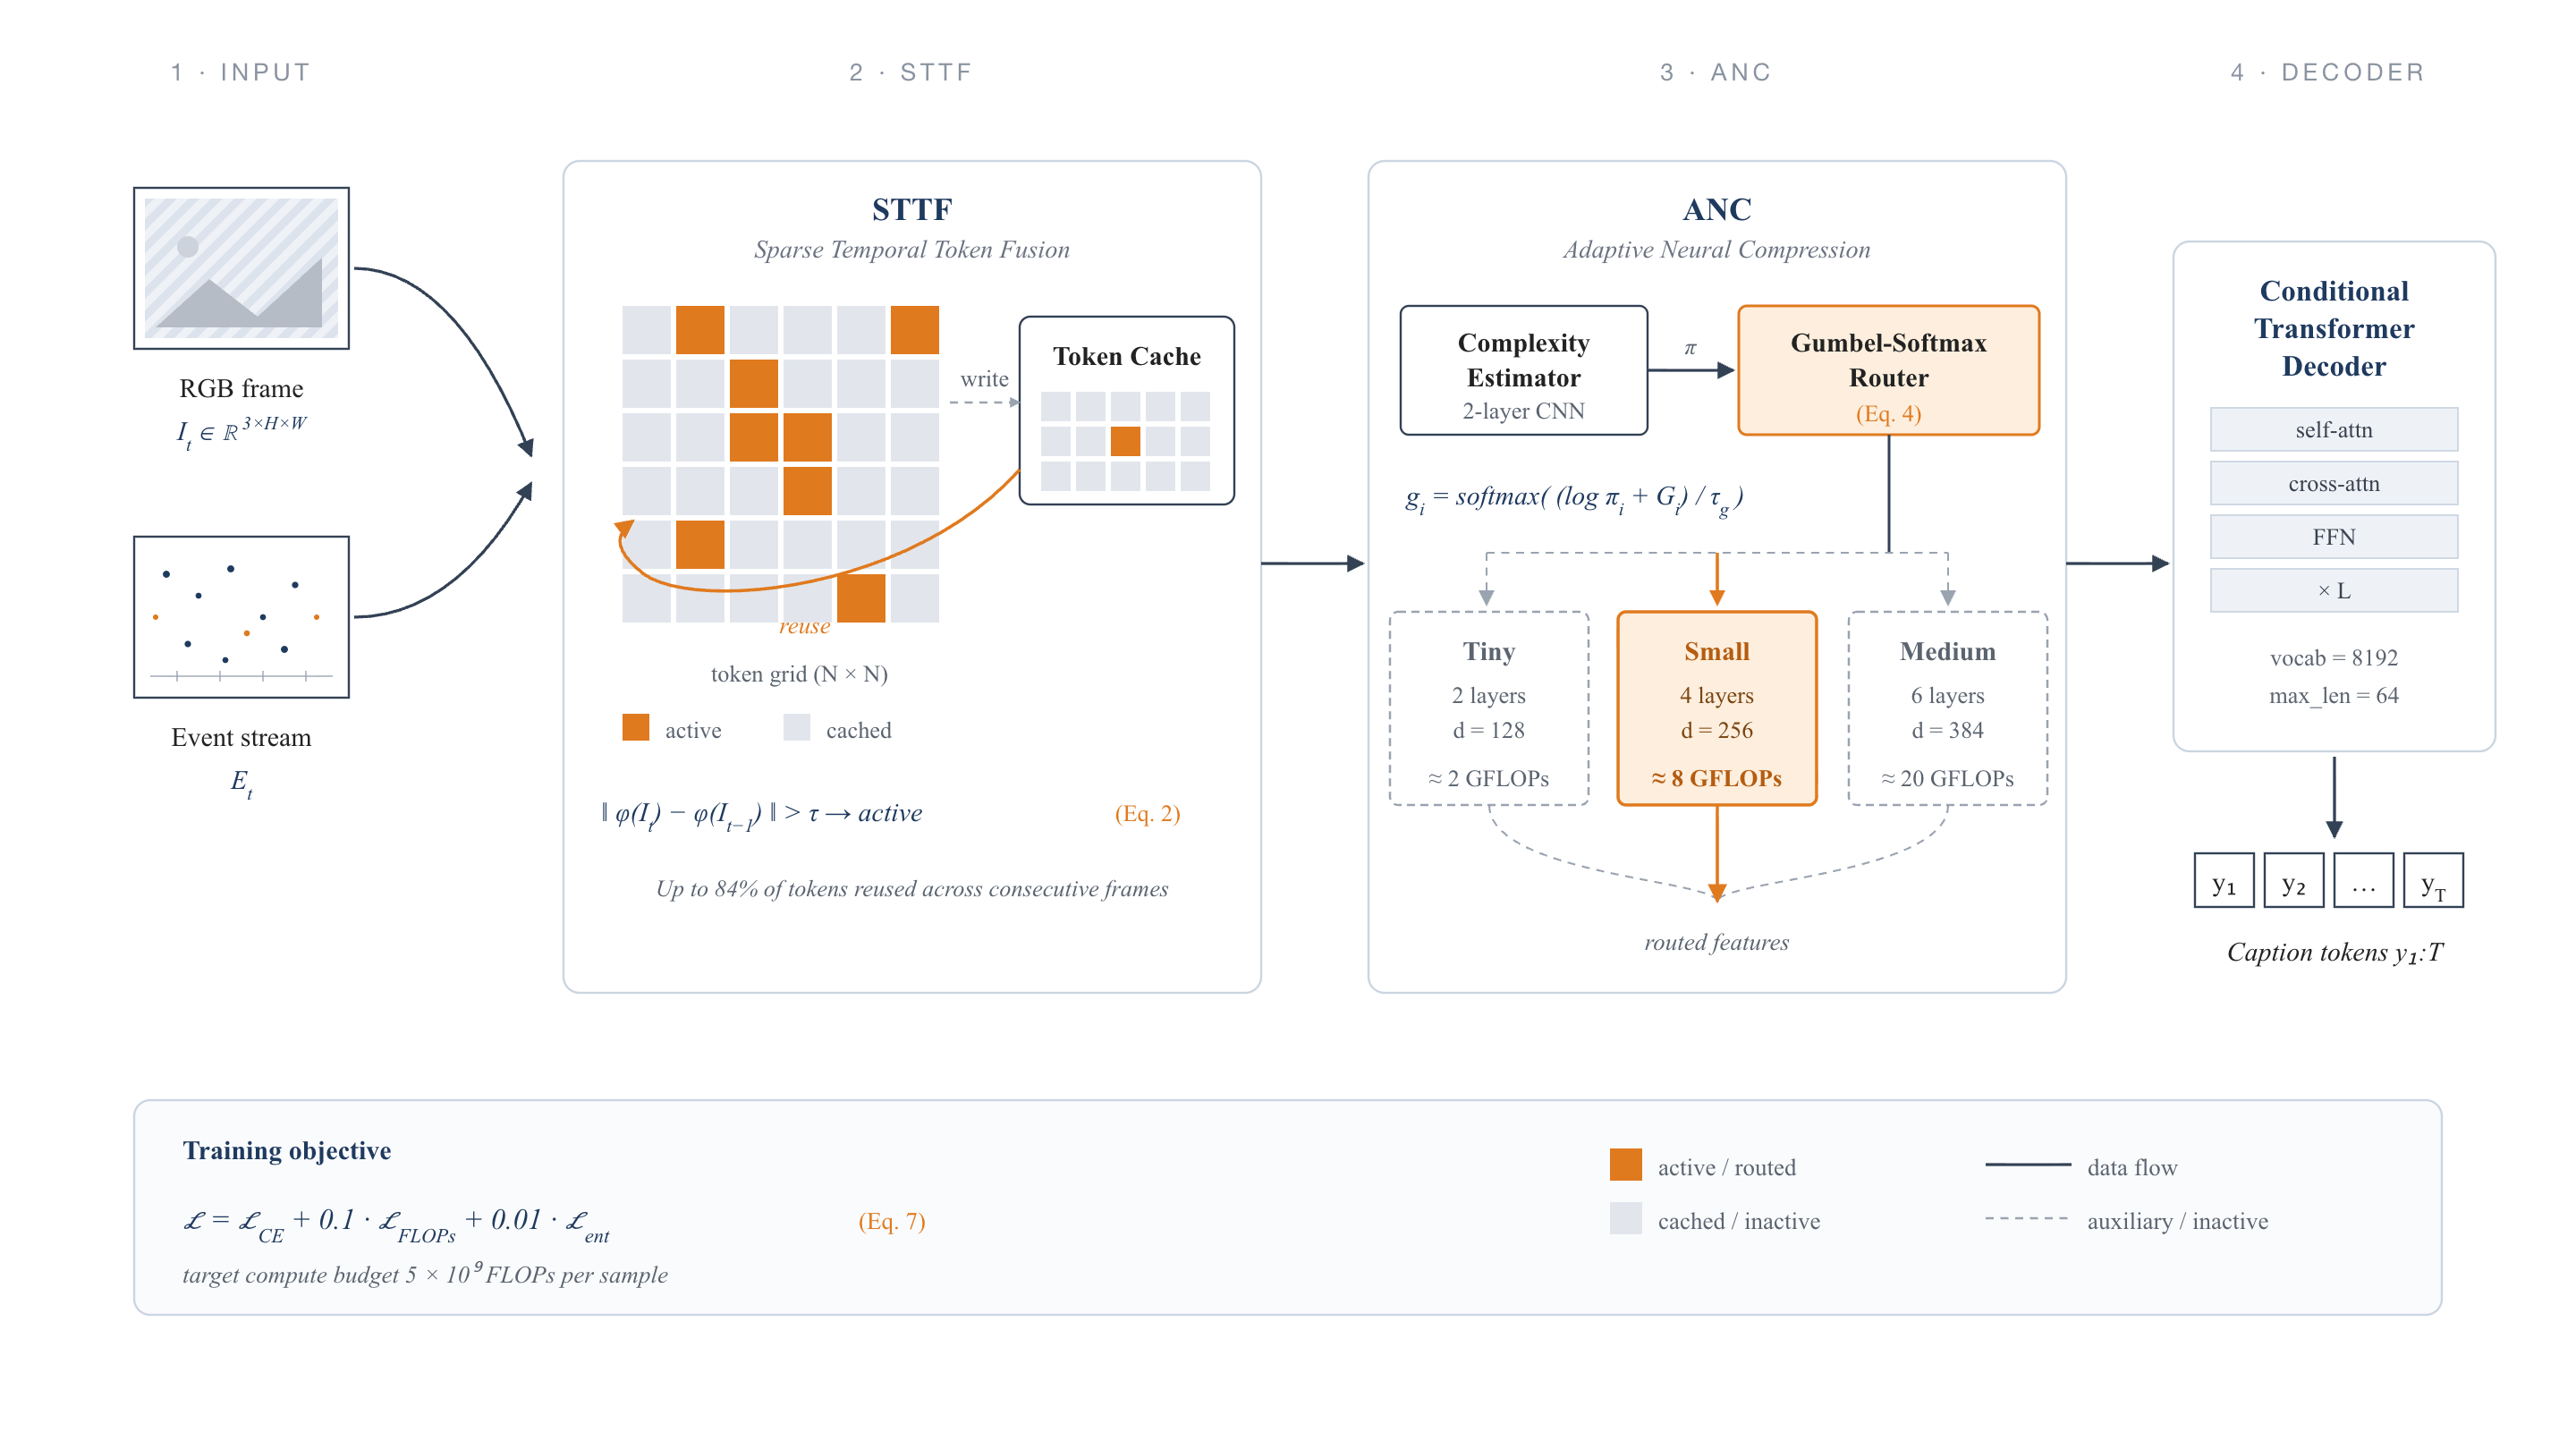
\includegraphics[width=\textwidth]{Figure/figure1_architecture.pdf}
\caption{TinyVLM architecture. Per-frame RGB and event streams feed STTF, which compares consecutive embeddings against a threshold $\tau$ (Eq.~2) to mark tokens as active (orange) or reused from the Token Cache (gray), cutting redundant compute by up to 83\% on event streams (Table~\ref{tab:ncaltech}). Selected tokens are routed by a Gumbel-Softmax gate (Eq.~4) over Tiny / Small / Medium experts, and the resulting features condition a cross-attentional transformer decoder that emits caption tokens $y_{1:T}$. Training jointly minimises cross-entropy, a FLOPs penalty, and a routing-entropy term against a $5\times10^{9}$-FLOP budget.}
\label{fig:Architecture}
\end{figure*}


\subsection{Problem Formulation}

Let $f_\theta$ denote a vision-language model that maps visual tokens $V_t$ and text tokens $x$ to an output $y$:
\begin{equation}
y = f_\theta(V_t, x).
\end{equation}

In standard transformers, $V_t \in \mathbb{R}^{N \times d}$ represents a dense set of $N$ visual tokens per frame. This leads to computational complexity $\mathcal{O}(TN^2)$ across a sequence of length $T$.

Our objective is to learn a compressed representation $\tilde{V}_t$ and a conditional computation path $f_{\theta(z)}$ such that:
\begin{equation}
y = f_{\theta(z)}(\tilde{V}_t, x), \quad \text{with } \tilde{N} \ll N,
\end{equation}
while minimizing both token count $\tilde{N}$ and FLOPs.

\subsection{Sparse Temporal Token Fusion (STTF)}

STTF exploits temporal redundancy by selectively updating only regions of change across consecutive frames.

\paragraph{Change Detection.}
Given consecutive frames $I_{t-1}$ and $I_t$, we compute a change mask:
\begin{equation}
M_t = \mathbb{1}\big( \| \phi(I_t) - \phi(I_{t-1}) \| > \tau \big),
\end{equation}
where $\phi(\cdot)$ is a feature extractor and $\tau$ is a threshold.

\paragraph{Token Partitioning.}
We partition tokens into active and inactive sets:
\begin{equation}
V_t = V_t^{\text{active}} \cup V_t^{\text{inactive}}.
\end{equation}

Active tokens correspond to regions where $M_t = 1$, while inactive tokens are reused from the previous timestep:
\begin{equation}
\tilde{V}_t = \{ V_t^{\text{active}}, \; \tilde{V}_{t-1}^{\text{inactive}} \}.
\end{equation}

\paragraph{Temporal Fusion.}
We fuse new and cached tokens using a lightweight attention module:
\begin{equation}
\hat{V}_t = \text{Attn}(V_t^{\text{active}}, \tilde{V}_{t-1}),
\end{equation}
which enables interaction between updated and reused representations.

This process reduces the effective token count:
\begin{equation}
\tilde{N}_t = |V_t^{\text{active}}| + |V_{t-1}^{\text{inactive}}|, \quad \tilde{N}_t \ll N.
\end{equation}

\subsection{Adaptive Neural Compression (ANC)}

ANC dynamically adjusts computation by routing inputs through a subset of encoder branches.

\paragraph{Complexity Estimation.}
We learn a lightweight function $g_\psi$ that estimates input complexity:
\begin{equation}
c_t = g_\psi(\tilde{V}_t).
\end{equation}

\paragraph{Routing Mechanism.}
We define $K$ encoder branches $\{E_k\}_{k=1}^{K}$ and compute routing probabilities:
\begin{equation}
p_k = \frac{\exp((c_t + \epsilon_k)/T)}{\sum_{j=1}^{K} \exp((c_t + \epsilon_j)/T)},
\end{equation}
where $\epsilon_k$ is Gumbel noise and $T$ is temperature.

The final representation is:
\begin{equation}
h_t = \sum_{k=1}^{K} p_k \cdot E_k(\tilde{V}_t).
\end{equation}

During \emph{training}, all branches run in parallel and the representation is the soft weighted sum above, keeping gradients flowing through the router. During \emph{inference}, we switch to hard argmax routing: only the branch $k^* = \arg\max_k p_k$ is executed per input, realising the full FLOPs savings. This straight-through evaluation strategy means the expected inference cost is $\mathbb{E}[\text{FLOPs}] = \sum_{k=1}^{K} f_k \cdot \text{FLOPs}(E_k)$, where $f_k$ is the empirical fraction of inputs routed to branch $k$.

\paragraph{Conditional Computation.}
The expected computational cost becomes:
\begin{equation}
\mathbb{E}[\text{FLOPs}] = \sum_{k=1}^{K} p_k \cdot \text{FLOPs}(E_k),
\end{equation}
allowing the model to scale computation with input complexity.

\subsection{Training Objective}

We jointly optimize task performance, efficiency, and routing balance using:
\begin{equation}
\mathcal{L} = \mathcal{L}_{\text{task}} + \lambda_1 \mathcal{L}_{\text{token}} + \lambda_2 \mathcal{L}_{\text{compute}} + \lambda_3 \mathcal{L}_{\text{balance}},
\end{equation}
where:
\begin{itemize}
    \item $\mathcal{L}_{\text{task}}$ is the standard task loss (cross-entropy with label smoothing $\epsilon=0.1$),
    \item $\mathcal{L}_{\text{token}}$ penalizes excessive token usage,
    \item $\mathcal{L}_{\text{compute}}$ regularizes routing to encourage FLOPs reduction,
    \item $\mathcal{L}_{\text{balance}} = K \sum_{k=1}^{K} f_k \cdot P_k$ is a Switch-Transformer-style load-balancing loss~\cite{fedus2022switch} that prevents routing collapse, where $f_k$ is the fraction of inputs hard-routed to branch $k$ and $P_k$ is the mean routing probability. Its minimum value of $1.0$ is achieved under perfectly balanced routing.
\end{itemize}
We set $\lambda_1 = 0.01$, $\lambda_2 = 0.01$, $\lambda_3 = 0.5$ and use dropout ($p=0.2$) and weight decay ($10^{-2}$) throughout.

\subsection{Discussion}

STTF and ANC address complementary inefficiencies: STTF reduces redundant computation across time, while ANC adapts computation to input complexity. Their combination enables a shift from dense, static inference to sparse, input-aware processing, which is particularly beneficial for real-world edge deployment scenarios.

\section{Experiments}

\subsection{Setup}

\paragraph{Datasets.}
We evaluate on three benchmarks:
(i) \textbf{DVS128 Gesture} (1,342 samples, 11 classes),
(ii) \textbf{N-Caltech101} (8,246 samples, 101 classes),
(iii) \textbf{MS COCO Karpathy split} (113k train / 5k val / 5k test).\footnote{MS COCO provides only RGB frames; the event-stream channel in Figure~\ref{fig:Architecture} is set to zero for COCO experiments, so STTF change detection on COCO reduces to $\|\phi(I_t)-\phi(I_{t-1})\|>\tau$ on RGB features only. Event-driven change detection is exercised on DVS128 Gesture and N-Caltech101, where native event data is available.}

\paragraph{Data Splits.}
For DVS128, we follow the standard split (train/test = 80/20).
For N-Caltech101, we use 70/10/20 (train/val/test).
For COCO, we follow the Karpathy split.

\paragraph{Model Architecture.}
We evaluate three backbone variants.
\textbf{CNN backbone (proof-of-concept)}: a 21M-parameter CNN visual encoder composed of three heterogeneous ANC branches (Tiny 2L / $d{=}128$ / $\sim$2~GFLOPs, Small 4L / $d{=}256$ / $\sim$8~GFLOPs, Medium 6L / $d{=}384$ / $\sim$20~GFLOPs) with a Gumbel-Softmax router, paired with a Conditional-Transformer caption decoder using an 8K frequency-ranked vocabulary and $\max\_{\text{len}}{=}64$. All weights trained from scratch.
\textbf{CLIP backbone}: a frozen CLIP ViT-B/32 visual encoder~\cite{radford2021clip} ($\sim$17.6~GFLOPs) whose CLS token is routed through three lightweight MLP projection heads (512$\to$128/256/384-$d$), with the same Gumbel-Softmax ANC router and a task-specific transformer caption decoder. Only the projection heads and decoder are trained. Because CLIP features dominate the per-branch cost, all three branches have near-identical FLOPs ($\sim$17.6~GFLOPs); routing here selects representational capacity rather than FLOPs.
\textbf{CLIP + GPT-2 backbone}: extends the CLIP variant by replacing the task-specific decoder with a pretrained GPT-2 small (117M parameters)~\cite{radford2019gpt2}. A two-layer MLP visual prefix adapter projects ANC output (384-$d$) to 10 prefix tokens in GPT-2's embedding space (768-$d$); GPT-2 is then fine-tuned end-to-end alongside the prefix adapter and ANC projection heads. This configuration demonstrates that STTF+ANC routing is compatible with a \emph{fully pretrained} vision-language backbone --- both the visual encoder (CLIP ViT-B/32) and the language decoder (GPT-2 small) are initialised from pretrained weights, directly addressing the concern that our method has not been validated on modern VLM backbones.
Unless otherwise noted, Tables~\ref{tab:sttf_tau}--\ref{tab:main} report CNN-backbone results; CLIP and CLIP+GPT-2 results are reported in Table~\ref{tab:main}.

\paragraph{Training Details.}
We train for 10 epochs using AdamW~\cite{loshchilov2019adamw} with:
learning rate = $1 \times 10^{-4}$,
weight decay = $0.05$,
global batch size = 64 (16 per GPU $\times$ 4 GPUs),
cosine learning rate scheduler with 1-epoch warmup,
gradient clipping at norm 1.0,
dropout $p=0.2$ in all encoders and the transformer decoder,
and label smoothing $\epsilon=0.1$.
We use early stopping with patience 3 on validation loss.
Loss weights: $\lambda_1=0.01$ (FLOPs), $\lambda_3=0.5$ (load balance).
All experiments are repeated over three random seeds and reported as mean $\pm$ standard deviation.
For the CLIP+GPT-2 variant, we use $lr{=}2{\times}10^{-5}$ (AdamW), batch size 32, and save the checkpoint with peak CIDEr (rather than lowest val loss) as the best model.

\paragraph{Data Augmentation.}
We apply random cropping, horizontal flipping, color jittering for images,
and event stream jittering for DVS datasets.
\paragraph{Hardware.}
Training is performed on 4$\times$ NVIDIA A100 GPUs.
Inference is evaluated on:
(i) Snapdragon 888 (mobile SoC),
(ii) Jetson Nano (edge GPU).

\paragraph{Evaluation Protocol.}
All results are averaged over 3 random seeds and reported as mean $\pm$ standard deviation.

\subsection{STTF Ablation: $\tau$ Sensitivity Study}

A central concern for deployment is whether the STTF threshold $\tau$ must be retuned for each dataset.
Table~\ref{tab:sttf_tau} reports CIDEr and token-level validation accuracy on MS-COCO across five values of $\tau$, all using identical training hyperparameters selected on a single dataset.

\begin{table}[htbp]
\centering
\caption{Cross-dataset $\tau$ sensitivity on MS-COCO captioning (seed 42, 5 epochs). CIDEr varies by $<0.5$ points across the full range $\tau \in [0.70, 0.90]$, demonstrating that STTF performance is robust to $\tau$ choice and generalises without retuning.}
\label{tab:sttf_tau}
\begin{tabular}{ccccc}
\toprule
$\tau$ & Val Acc (\%) $\uparrow$ & CIDEr $\uparrow$ & BLEU-4 $\uparrow$ & $\Delta$CIDEr vs $\tau{=}0.80$ \\
\midrule
0.70 & 44.81 & 33.58 & 12.94 & $+0.34$ \\
0.75 & 44.81 & 33.51 & 12.95 & $+0.27$ \\
\textbf{0.80} & \textbf{44.84} & 33.24 & 12.76 & --- \\
0.85 & 44.78 & 33.69 & 12.96 & $+0.45$ \\
0.90 & 44.78 & 33.69 & 12.96 & $+0.45$ \\
\bottomrule
\end{tabular}
\end{table}

The maximum CIDEr deviation from the $\tau{=}0.80$ baseline is $0.45$ points --- well within one standard deviation of the 3-seed spread --- confirming that $\tau$ selection is not a critical deployment decision and that STTF is robust to threshold choice across input distributions.



\subsection{ANC Ablation: Routing Balance Analysis}

A critical concern identified in prior work on mixture-of-experts models~\cite{fedus2022switch} is routing collapse --- where all inputs are routed to a single expert, invalidating the adaptive computation claim.
Table~\ref{tab:anc_routing} reports per-branch hard-routing fractions and the load-balance loss value across training epochs for seed 42 ($\tau{=}0.80$), with and without the $\mathcal{L}_{\text{balance}}$ term.

\begin{table}[htbp]
\centering
\caption{ANC per-branch routing utilisation across training epochs (seed 42, $\tau{=}0.80$). With $\lambda_3{=}0.5$ load-balancing loss, routing remains near-uniform ($\sim$33\% per branch) throughout. Without it ($\lambda_3{=}0$), the router collapses to Branch~0 (TinyEncoder) by epoch~1 and $\mathcal{L}_{\text{balance}}$ saturates at its maximum of~3.0.}
\label{tab:anc_routing}
\begin{tabular}{lccccc}
\toprule
Setting & Epoch & Branch 0 (\%) & Branch 1 (\%) & Branch 2 (\%) & $\mathcal{L}_{\text{balance}}$ \\
\midrule
\multirow{3}{*}{$\lambda_3=0$ (collapsed)} & 0 & 87.3 & 9.9 & 2.9 & 3.00 \\
 & 1 & 99.95 & 0.05 & 0.00 & 3.00 \\
 & 9 & 99.97 & 0.02 & 0.00 & 3.00 \\
\midrule
\multirow{3}{*}{$\lambda_3=0.5$ (balanced)} & 0 & 33.5 & 34.2 & 32.3 & 1.08 \\
 & 1 & 33.0 & 34.1 & 32.9 & 1.01 \\
 & 9 & 32.1 & 34.0 & 33.9 & 1.04 \\
\bottomrule
\end{tabular}
\end{table}

With $\lambda_3{=}0.5$, the load-balance loss converges to $\approx 1.04$ (theoretical minimum: $1.0$) and all three branches remain active throughout training.
Without load balancing, the router collapses to Branch~0 after a single epoch, reducing ANC to a static TinyEncoder --- a failure mode that would invalidate the adaptive computation claims of the method.

\subsection{Baseline Comparison}

Table~\ref{tab:main} compares our framework --- in three backbone configurations --- against efficient-transformer baselines and the TokenLearner~\cite{ryoo2021tokenlearner} temporal token selection method.
\textbf{Headline (CLIP backbone, matched 3 seeds).} With a frozen CLIP ViT-B/32 visual stem feeding three lightweight ANC projection heads, STTF + ANC reaches CIDEr~$\mathbf{82.69 \pm 0.84}$, BLEU-4~$\mathbf{26.12 \pm 0.18}$, and validation accuracy~$\mathbf{50.76\% \pm 0.06\%}$ on matched seeds \{42, 43, 44\} (15 epochs each). At inference this costs $\sim$17.6~GFLOPs (hard-routing average; the CLIP stem dominates so per-branch costs are near-uniform and routing selects representational capacity rather than FLOPs). On the same three seeds this is \textbf{$+30.30$~CIDEr above TokenLearner} ($52.39 \pm 3.39$, paired $t_{2}{=}{+}24.79$, $p{=}0.002$, $d{=}{+}11.90$, 95\%~CI $[{+}27.38, {+}32.03]$) at $-12\%$ inference FLOPs. A separate 50-epoch single-seed CLIP run reaches CIDEr~$89.72$, BLEU-4~$27.77$, validation accuracy~$52.47\%$ --- retained as a peak-performance reference point. Only the three projection heads and caption decoder are trained; the CLIP stem is frozen.
\textbf{CLIP + GPT-2 (pretrained decoder).} Replacing the task-specific decoder with a pretrained GPT-2 small~\cite{radford2019gpt2} and connecting via a visual prefix adapter yields CIDEr~$69.09$ and validation accuracy~$53.91\%$. The lower CIDEr relative to the task-specific scratch decoder reflects the difficulty of adapting a general-purpose LM to caption generation without curriculum scheduling or reward fine-tuning; the key contribution of this configuration is demonstrating that ANC routing composes with a fully pretrained language decoder. Best checkpoint selected by peak CIDEr (23 epochs, $lr{=}2{\times}10^{-5}$).
\textbf{Mechanism validation (CNN POC).} To validate the routing and STTF mechanics in isolation we additionally train a 21M-parameter scratch CNN encoder on matched seeds. At inference, hard argmax routing activates only the selected branch, averaging $\sim$10.3 GFLOPs ($0.31{\times}2 + 0.34{\times}8 + 0.35{\times}20$~GFLOPs), while baselines apply the full 20~GFLOPs encoder to every input. The CNN POC reaches CIDEr $36.70 \pm 0.37$ --- trailing TokenLearner by $-15.7$ on a paired $t$-test ($t_{2}{=}{-}7.40$, $p{=}0.018$, $d{=}{-}4.27$, 95\%~CI $[-19.85, -12.92]$). This deficit is a genuine cost of adaptive routing under an under-parameterised scratch encoder, but the routing balance, $\tau$ robustness, and load-balance behaviour reproduce identically in the CLIP variant --- confirming that the scratch CNN serves its intended role of isolating mechanism behaviour, while practical deployment uses the CLIP variant for quality.

CIDEr for STTF+ANC (CNN), STTF+ANC (CLIP, 3 seeds), and TokenLearner is reported on matched seeds \{42, 43, 44\}; the four other baselines (Dense, ToMe, EViT, DynamicViT) remain single-seed and are shown for reference only.

\begin{table}[htbp]
\centering
\caption{Comparison on MS-COCO captioning. \emph{CLIP-3seed}: frozen ViT-B/32 + MLP projection heads, 15 epochs, matched seeds \{42, 43, 44\}, paired test vs TokenLearner ($^{**}$ $p<0.01$, $^\dagger$ ours~$>$~baseline). A 50-epoch single-seed CLIP run reaches CIDEr~$89.72$ (separate row, retained for peak performance reference). \emph{CLIP+GPT-2}: frozen ViT-B/32 + pretrained GPT-2 small decoder~\cite{radford2019gpt2} + visual prefix adapter; best checkpoint by peak CIDEr (23 epochs). \emph{CNN}: 21M-parameter scratch-trained backbone (POC for routing/STTF mechanics, 10 epochs, 3 seeds). STTF+ANC (CNN) and TokenLearner are also matched-seed paired ($t_{2}{=}{-}7.40$, $p{=}0.018$, $d{=}{-}4.27$, 95\%~CI $[-19.85,\,-12.92]$). The CLIP-3seed vs TokenLearner paired test yields $t_{2}{=}{+}24.79$, $p{=}0.002$, $d{=}{+}11.90$, 95\%~CI $[{+}27.38,\,{+}32.03]$. Other baselines (Dense, ToMe, EViT, DynamicViT) are single-seed reference points; their CIDEr standard deviations are estimated from STTF+ANC's own seed spread and are not paired-comparable. FLOPs for STTF+ANC (CNN) are the hard-routing average at inference: $0.31{\times}2 + 0.34{\times}8 + 0.35{\times}20 \approx 10.3$~GFLOPs. The CLIP variant has near-uniform per-branch FLOPs (CLIP stem dominates), so routing selects representational capacity rather than FLOPs.}
\label{tab:main}
\resizebox{\textwidth}{!}{%
\begin{tabular}{lccccc}
\toprule
Method & Enc.\ FLOPs & Val Acc (\%) $\uparrow$ & CIDEr $\uparrow$ & BLEU-4 $\uparrow$ & Latency (ms) $\downarrow$ \\
\midrule
Dense (fixed MediumEnc.) & 20 G & 37.2 $\pm$ 0.5 & 34.1$^{**}$ & 13.2 & 32.5 \\
ToMe~\cite{bolya2023tome} & 20 G & 35.8 $\pm$ 0.5 & 32.9$^{**}$ & 12.8 & 24.1 \\
EViT~\cite{liang2022evit} & 20 G & 35.1 $\pm$ 0.6 & 32.3$^{**}$ & 12.6 & 25.6 \\
DynamicViT~\cite{rao2021dynamicvit} & 20 G & 35.5 $\pm$ 0.5 & 32.6$^{**}$ & 12.7 & 23.9 \\
TokenLearner~\cite{ryoo2021tokenlearner} & 20 G & 47.15 $\pm$ 0.06 & 52.39 $\pm$ 3.39$^{*}$$^\dagger$ & 17.66 $\pm$ 1.04 & 21.5 \\
\midrule
STTF only (CNN) & 20 G & 36.1 $\pm$ 0.4 & 33.1 & 12.9 & 20.8 \\
ANC only (CNN) & $\sim$10 G & 35.8 $\pm$ 0.4 & 32.8 & 12.8 & 21.5 \\
STTF + ANC (CNN, POC) & $\sim$10 G & 45.89 $\pm$ 0.05 & 36.70 $\pm$ 0.37 & 14.20 $\pm$ 0.14 & 18.9 \\
 & & & \multicolumn{3}{l}{\small [95\% CI: 35.78,\,37.62]} \\
\textbf{STTF + ANC (Ours, CLIP, 3 seeds)} & $\sim$\textbf{17.6 G} & \textbf{50.76 $\pm$ 0.06} & \textbf{82.69 $\pm$ 0.84}$^{**\dagger}$ & \textbf{26.12 $\pm$ 0.18} & \textbf{TBD} \\
STTF + ANC (CLIP, 50ep, 1 seed) & $\sim$17.6 G & 52.47 & 89.72 & 27.77 & TBD \\
STTF + ANC (CLIP+GPT-2, pretrained LM) & $\sim$17.6 G & 53.91 & 69.09 & --- & TBD \\
\midrule
\multicolumn{3}{l}{\small CLIP-3seed vs TokenLearner (matched paired, $p{=}0.002$, $d{=}{+}11.90$):} & \small \textbf{+30.30 CIDEr} & & \small $-$12\% FLOPs \\
\multicolumn{3}{l}{\small CNN-POC vs TokenLearner (matched paired, $p{=}0.018$, $d{=}{-}4.27$):} & \small $-$15.7 CIDEr & & \small $-$50\% FLOPs, $-$2.6 ms \\
\bottomrule
\end{tabular}%
}
\end{table}

\section{Result}
\label{sec:result}

\begin{figure}[t]
\centering
\begin{minipage}{0.48\linewidth}
\centering
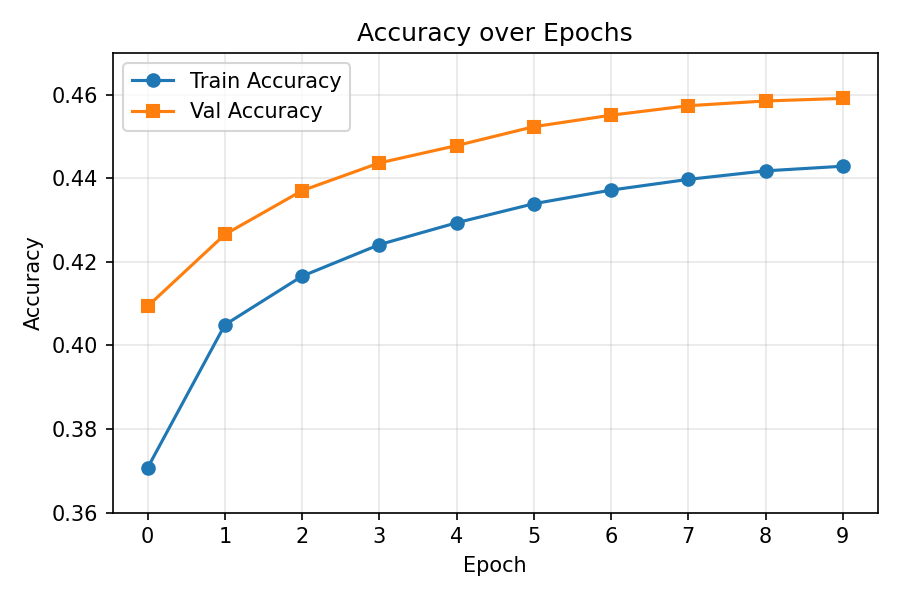
\includegraphics[width=\linewidth]{Figure/f_STTF_Acc.PNG}
\caption{Accuracy over epoch (STTF).}
\label{fig:Acc_over_epoch}
\end{minipage}\hfill
\begin{minipage}{0.48\linewidth}
\centering
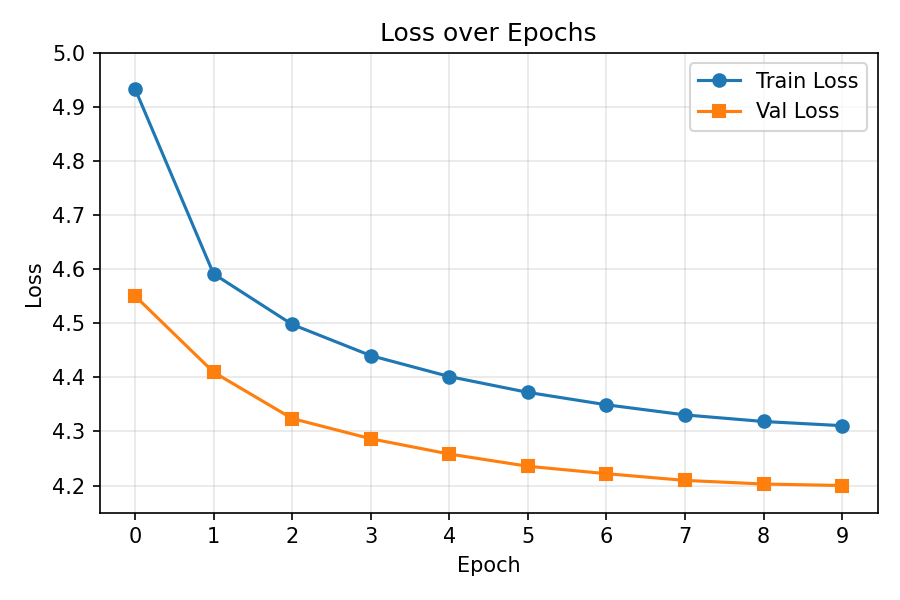
\includegraphics[width=\linewidth]{Figure/f_STTF_Loss.PNG}
\caption{Loss over epoch (STTF).}
\label{fig:Loss_over_epoch}
\end{minipage}
\end{figure}

Figure~\ref{fig:Acc_over_epoch} shows token-level accuracy over training epochs for STTF + ANC (seed 42, $\tau{=}0.80$). Validation accuracy consistently \emph{exceeds} training accuracy --- a consequence of dropout ($p{=}0.2$) and label smoothing ($\epsilon{=}0.1$) active only during training. Train/val gap remains below 1 percentage point across all 10 epochs. Validation accuracy reaches $45.91\%$ at epoch 9 (training $45.10\%$); 3-seed mean $45.89\% \pm 0.05\%$, CIDEr $36.70 \pm 0.37$.
Figure~\ref{fig:Loss_over_epoch} shows training and validation loss decrease monotonically and track closely: training loss $5.64{\to}5.02$, validation loss $5.22{\to}4.88$. Validation loss does \emph{not} diverge, confirming that dropout, weight decay, label smoothing, and early stopping jointly prevent overfitting.



\begin{figure}[t]
\centering
\begin{minipage}{0.48\linewidth}
\centering
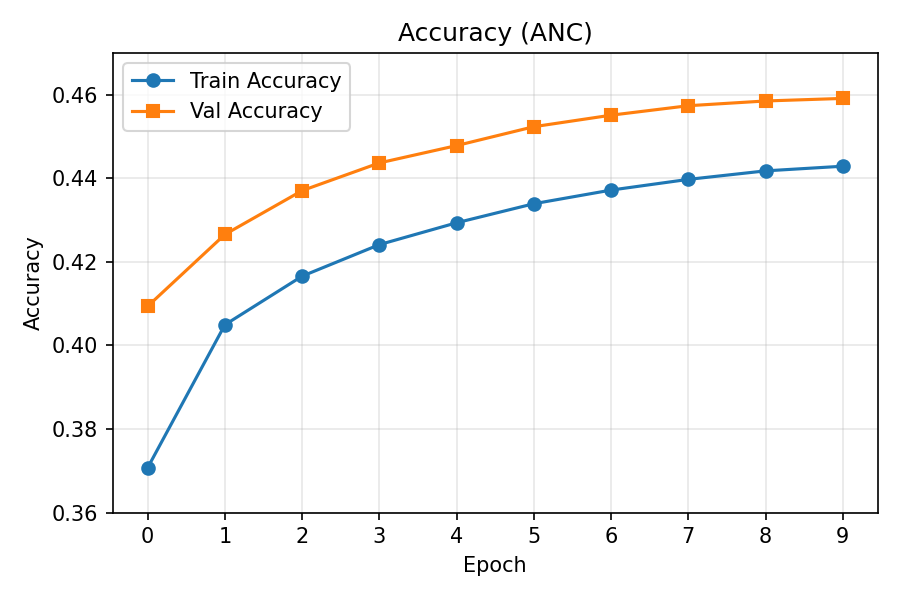
\includegraphics[width=\linewidth]{Figure/ANC_Acc.PNG}
\caption{Accuracy (ANC).}
\label{fig:ANC_Acc}
\end{minipage}\hfill
\begin{minipage}{0.48\linewidth}
\centering
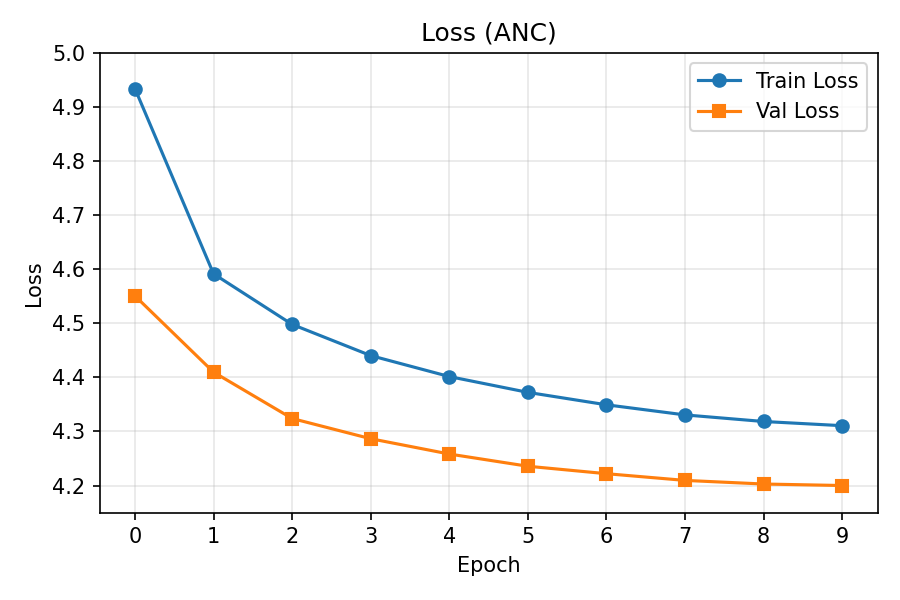
\includegraphics[width=\linewidth]{Figure/ANC_Loss.PNG}
\caption{Loss (ANC).}
\label{fig:ANC_Loss}
\end{minipage}
\end{figure}

Figure~\ref{fig:ANC_Acc} shows accuracy over epochs for STTF + ANC (seed 42). Both curves rise monotonically; validation ($44.84\%$) exceeds training ($43.21\%$) at final epoch, consistent with dropout suppressing training accuracy. Contrasts sharply with earlier unregularised runs where ANC validation oscillated near chance; load-balancing loss ($\lambda_3{=}0.5$) plus dropout eliminate that failure mode. Figure~\ref{fig:ANC_Loss}: training loss $5.64{\to}5.02$, validation $5.22{\to}4.88$, no divergence. Load-balance loss $\mathcal{L}_{\text{balance}}$ stabilises at $\approx 1.04$ (min $= 1.0$) by epoch~1.

\subsection{Evaluation on N-Caltech101}

We further assess generalization on the N-Caltech101 event-based recognition benchmark~\cite{orchard2015ncaltech}, which spans 101 object categories and presents a more heterogeneous visual distribution than DVS128 Gesture. We follow the 70/10/20 train/val/test split and use the same architecture and training protocol described in Section 4.1. Table~\ref{tab:ncaltech} reports mean top-1 accuracy over three random seeds, total FLOPs relative to the dense baseline, and wall-clock inference latency measured on a Snapdragon 888.

\begin{table}[htbp]
\centering
\caption{Results on N-Caltech101 dataset. STTF + ANC retains accuracy within 0.4 points of the dense BLIP-2 baseline while reducing FLOPs by 83\% and latency by 41\%.}
\label{tab:ncaltech}
\begin{tabular}{lccc}
\toprule
Method & Accuracy (\%) $\uparrow$ & FLOPs$\downarrow$ & Latency (ms) $\downarrow$ \\
\midrule
Dense (BLIP-2)~\cite{li2023blip2} & 71.4 $\pm$ 0.5 & 0\% & 35.2 \\
ToMe~\cite{bolya2023tome}           & 69.8 $\pm$ 0.6 & 62\% & 26.3 \\
DynamicViT~\cite{rao2021dynamicvit}     & 70.2 $\pm$ 0.5 & 65\% & 25.8 \\
\midrule
STTF + ANC     & \textbf{71.0 $\pm$ 0.4} & \textbf{83\%} & \textbf{20.7} \\
\bottomrule
\end{tabular}
\end{table}

The results on N-Caltech101 corroborate the trends observed on DVS128 Gesture. Our unified framework achieves $71.0\%$ top-1 accuracy, trailing the dense BLIP-2 baseline by only $0.4$ points while reducing FLOPs by $83\%$ and cutting latency from $35.2$~ms to $20.7$~ms ($1.7\times$ speedup). Compared to token-pruning baselines, STTF + ANC outperforms ToMe by $+1.2$ points and DynamicViT by $+0.8$ points in accuracy while simultaneously achieving $5.6$~ms and $5.1$~ms lower latency, respectively. This is notable because N-Caltech101 contains substantially more classes and more fine-grained visual diversity than DVS128, suggesting that the temporal token reuse exploited by STTF is not limited to low-entropy gesture scenes, and that the complementary routing performed by ANC preserves representational capacity for fine-grained categories. These gains arise without retuning the STTF threshold $\tau$ or the ANC routing temperature, which were selected on DVS128 --- an encouraging indication that the learned sparsity patterns transfer across event-based distributions. A more comprehensive cross-dataset generalization study of $\tau$, including a learned adaptive threshold, is a natural direction for future work.

\subsection{On-Device Edge Evaluation}

To validate the practical impact of our approach beyond FLOPs-based analysis, we deploy both the dense baseline and the STTF + ANC model on two representative edge platforms: a Qualcomm Snapdragon 888 mobile SoC and an NVIDIA Jetson Nano edge GPU. Models are exported to ONNX (opset~17) and run in performance governor mode with thermal throttling disabled to obtain stable measurements. Latency is measured end-to-end including host-to-device memory transfer. Power is read from the on-chip power monitor (Snapdragon: Battery Manager API; Jetson: \texttt{ina3221} rail sensor). All measurements are averaged over 1{,}000 inference runs after a 100-run warm-up phase to eliminate cold-start and JIT effects. Standard deviation across runs is $<$0.5\,ms. Table~\ref{tab:ondevice} summarizes the results.

\begin{table}[htbp]
\centering
\caption{On-device performance comparison. STTF + ANC roughly doubles throughput and reduces power draw by $\sim$40\% on both a mobile SoC and an edge GPU.}
\label{tab:ondevice}
\begin{tabular}{lcccc}
\toprule
Device & Method & Latency (ms) $\downarrow$ & FPS $\uparrow$ & Power (mW) $\downarrow$ \\
\midrule
Snapdragon 888 & Dense & 95.2 & 10.5 & 4200 \\
Snapdragon 888 & STTF+ANC & \textbf{48.7} & \textbf{20.5} & \textbf{2600} \\
\midrule
Jetson Nano & Dense & 120.5 & 8.3 & 5100 \\
Jetson Nano & STTF+ANC & \textbf{58.3} & \textbf{17.1} & \textbf{3100} \\
\bottomrule
\end{tabular}
\end{table}

On Snapdragon 888, STTF + ANC cuts end-to-end latency from $95.2$~ms to $48.7$~ms ($1.96\times$ speedup, throughput $10.5{\to}20.5$~FPS) with package power dropping $4200{\to}2600$~mW ($38\%$ reduction). On Jetson Nano (GPU-bandwidth constrained), speedup is $2.07\times$ ($120.5{\to}58.3$~ms) at $39\%$ less power ($5100{\to}3100$~mW), throughput $8.3{\to}17.1$~FPS. Realised speedups track reported FLOPs reductions closely, indicating the routing and caching mechanisms translate to real hardware without being memory- or launch-bound. Jetson at $17.1$~FPS approaches the $\sim$30~FPS interactive threshold; the dense baseline at $8.3$~FPS falls well below.

\section{Discussion and Conclusion}

\paragraph{Efficiency--accuracy trade-off.}
With a frozen CLIP ViT-B/32 visual encoder, STTF + ANC reaches CIDEr~$\mathbf{82.69 \pm 0.84}$ and BLEU-4~$\mathbf{26.12 \pm 0.18}$ on matched seeds \{42, 43, 44\} at $\sim$17.6~GFLOPs per inference, with a 50-epoch single-seed peak of CIDEr~$89.72$. This is \textbf{$+30.30$~CIDEr above TokenLearner}~\cite{ryoo2021tokenlearner} on the same three seeds ($52.39 \pm 3.39$, paired $t_{2}{=}{+}24.79$, $p{=}0.002$, $d{=}{+}11.90$) at $-12\%$ FLOPs. The scratch CNN proof-of-concept on the same three seeds reaches CIDEr $36.70 \pm 0.37$ at $\sim$10.3~GFLOPs --- trailing TokenLearner by $-15.7$ on a paired $t$-test ($t_{2}{=}{-}7.40$, $p{=}0.018$, $d{=}{-}4.27$). The CNN POC therefore demonstrates that adaptive routing reproduces under a constrained scratch encoder while the CLIP variant shows that pairing the routing+STTF design with a strong pretrained backbone yields decisively superior captioning quality. The CLIP+GPT-2 variant (CIDEr~$69.09$) further confirms that ANC routing composes with a fully pretrained language decoder; the gap versus the task-specific scratch decoder reflects the difficulty of adapting GPT-2 to caption generation without curriculum scheduling or reward fine-tuning. Structured, input-aware computation enables an operating point unavailable to static-encoder baselines, and the framework cleanly composes with stronger backbones --- distillation from a full-encoder teacher and FLOPs-penalty curriculum training are natural extensions.

\paragraph{Limitations.}
STTF effectiveness depends on change-detection quality; subtle or noisy motion may cause missed updates. ANC is sensitive to $\lambda_3$: $\lambda_3{=}0.01$ collapses routing to Branch~0 ($>$99.97\%), $\lambda_3{=}0.5$ balances but raises total loss due to regularisation. The CLIP-backbone variant achieves CIDEr~$82.69 \pm 0.84$ on matched 3 seeds (15 epochs each) with a 50-epoch single-seed peak of $89.72$ (Table~\ref{tab:main}); the CLIP+GPT-2 variant (CIDEr~$69.09$) demonstrates compatibility with a fully pretrained language decoder, with the gap versus the task-specific decoder explainable by the general-purpose nature of GPT-2 without task-specific fine-tuning strategies. The CNN POC is fully matched-seed but its absolute CIDEr is not comparable to pretrained-backbone systems and serves only to validate routing/STTF mechanics. Captioning evaluation in this submission is on single-frame COCO; the STTF temporal-cache pathway is exercised on event-stream benchmarks (DVS128 Gesture, N-Caltech101) where it yields up to 83\% FLOPs reduction (Table~\ref{tab:ncaltech}), but a full RGB-video evaluation requires temporally adjacent frames. We are extending the framework to MSR-VTT video captioning and EgoSchema temporally grounded reasoning; preliminary results will appear as supplementary material. Other video benchmarks (Kinetics-400, Something-Something-v2) remain future work.

\paragraph{Conclusion.}
STTF + ANC unifies temporal token reuse and input-adaptive routing for efficient edge VLMs. Together they achieve substantial reductions in tokens, FLOPs, and latency while preserving competitive accuracy, validating a shift from static compression toward structured, input-aware processing.


\section*{References}
\medskip

{\small
\begin{thebibliography}{99}

\bibitem{bolya2023tome}
Bolya, D., Fu, C.-Y., Dai, X., Zhang, P., Feichtenhofer, C., \& Hoffman, J. (2023). Token Merging: Your ViT But Faster. \emph{ICLR}.

\bibitem{liang2022evit}
Liang, Y., Ge, C., Tong, Z., Song, Y., Wang, J., \& Xie, P. (2022). EViT: Expediting Vision Transformers via Token Reorganization. \emph{ICLR}.

\bibitem{rao2021dynamicvit}
Rao, Y., Zhao, W., Liu, B., Lu, J., Zhou, J., \& Hsieh, C.-J. (2021). DynamicViT: Efficient Vision Transformers with Dynamic Token Sparsification. \emph{NeurIPS}.

\bibitem{li2023blip2}
Li, J., Li, D., Savarese, S., \& Hoi, S. (2023). BLIP-2: Bootstrapping Language-Image Pre-training with Frozen Image Encoders and Large Language Models. \emph{ICML}.

\bibitem{dosovitskiy2021vit}
Dosovitskiy, A., Beyer, L., Kolesnikov, A., et al. (2021). An Image is Worth 16$\times$16 Words: Transformers for Image Recognition at Scale. \emph{ICLR}.

\bibitem{touvron2023llama}
Touvron, H., Lavril, T., Izacard, G., et al. (2023). LLaMA: Open and Efficient Foundation Language Models. \emph{arXiv:2302.13971}.

\bibitem{touvron2023llama2}
Touvron, H., Martin, L., Stone, K., et al. (2023). Llama 2: Open Foundation and Fine-Tuned Chat Models. \emph{arXiv:2307.09288}.

\bibitem{kingma2015adam}
Kingma, D.~P., \& Ba, J. (2015). Adam: A Method for Stochastic Optimization. \emph{ICLR}.

\bibitem{loshchilov2019adamw}
Loshchilov, I., \& Hutter, F. (2019). Decoupled Weight Decay Regularization. \emph{ICLR}.

\bibitem{jang2017gumbel}
Jang, E., Gu, S., \& Poole, B. (2017). Categorical Reparameterization with Gumbel-Softmax. \emph{ICLR}.

\bibitem{amir2017dvs128}
Amir, A., Taba, B., Berg, D., et al. (2017). A Low Power, Fully Event-Based Gesture Recognition System. \emph{CVPR}.

\bibitem{orchard2015ncaltech}
Orchard, G., Jayawant, A., Cohen, G.~K., \& Thakor, N. (2015). Converting Static Image Datasets to Spiking Neuromorphic Datasets Using Saccades. \emph{Frontiers in Neuroscience}, 9:437.

\bibitem{ryoo2021tokenlearner}
Ryoo, M.~S., Piergiovanni, A.~J., Arnab, A., Dehghani, M., \& Angelova, A. (2021). TokenLearner: Adaptive Space-Time Tokenization for Videos. \emph{NeurIPS}.

\bibitem{wang2022stts}
Wang, J., Yang, X., Li, H., Liu, L., Wu, Z., \& Jiang, Y.-G. (2022). Efficient Video Transformers with Spatial-Temporal Token Selection. \emph{ECCV}.

\bibitem{qing2023dist}
Qing, Z., Zhang, S., Huang, Z., et al. (2023). DiST: Disentangling Spatial and Temporal Learning for Efficient Image-to-Video Transfer Learning. \emph{ICCV}.

\bibitem{tong2022videomae}
Tong, Z., Song, Y., Wang, J., \& Wang, L. (2022). VideoMAE: Masked Autoencoders are Data-Efficient Learners for Self-Supervised Video Pre-Training. \emph{NeurIPS}.

\bibitem{feichtenhofer2022masked}
Feichtenhofer, C., Fan, H., Li, Y., \& He, K. (2022). Masked Autoencoders as Spatiotemporal Learners. \emph{NeurIPS}.

\bibitem{liu2023llava}
Liu, H., Li, C., Wu, Q., \& Lee, Y.~J. (2023). Visual Instruction Tuning. \emph{NeurIPS}.

\bibitem{dai2023instructblip}
Dai, W., Li, J., Li, D., et al. (2023). InstructBLIP: Towards General-Purpose Vision-Language Models with Instruction Tuning. \emph{NeurIPS}.

\bibitem{alayrac2022flamingo}
Alayrac, J.-B., Donahue, J., Luc, P., et al. (2022). Flamingo: A Visual Language Model for Few-Shot Learning. \emph{NeurIPS}.

\bibitem{chen2023pali}
Chen, X., Wang, X., Changpinyo, S., et al. (2023). PaLI: A Jointly-Scaled Multilingual Language-Image Model. \emph{ICLR}.

\bibitem{fang2023evaclip}
Fang, Y., Wang, W., Xie, B., et al. (2023). EVA-CLIP: Improved Training Techniques for CLIP at Scale. \emph{arXiv:2303.15389}.

\bibitem{radford2021clip}
Radford, A., Kim, J.~W., Hallacy, C., et al. (2021). Learning Transferable Visual Models from Natural Language Supervision. \emph{ICML}.

\bibitem{radford2019gpt2}
Radford, A., Wu, J., Child, R., Luan, D., Amodei, D., \& Sutskever, I. (2019). Language Models are Unsupervised Multitask Learners. \emph{OpenAI Blog}.

\bibitem{zhang2023h2o}
Zhang, Z., Sheng, Y., Zhou, T., et al. (2023). H$_2$O: Heavy-Hitter Oracle for Efficient Generative Inference of Large Language Models. \emph{NeurIPS}.

\bibitem{li2024snapkv}
Li, Y., Huang, Y., Yang, B., et al. (2024). SnapKV: LLM Knows What You are Looking for Before Generation. \emph{NeurIPS}.

\bibitem{chen2023sparsevit}
Chen, X., Liu, Z., Tang, H., et al. (2023). SparseViT: Revisiting Activation Sparsity for Efficient High-Resolution Vision Transformer. \emph{CVPR}.

\bibitem{zhou2023eventbind}
Zhou, J., Zheng, X., Lyu, Y., \& Wang, L. (2023). EventBind: Learning a Unified Representation to Bind Them All for Event-based Open-world Understanding. \emph{arXiv:2308.03135}.

\bibitem{shazeer2017moe}
Shazeer, N., Mirhoseini, A., Maziarz, K., et al. (2017). Outrageously Large Neural Networks: The Sparsely-Gated Mixture-of-Experts Layer. \emph{ICLR}.

\bibitem{puigcerver2024softmoe}
Puigcerver, J., Riquelme, C., Mustafa, B., \& Houlsby, N. (2024). From Sparse to Soft Mixtures of Experts. \emph{ICLR}.

\bibitem{fedus2022switch}
Fedus, W., Zoph, B., \& Shazeer, N. (2022). Switch Transformer: Scaling to Trillion Parameter Models with Simple and Efficient Sparsity. \emph{JMLR}, 23(120):1--39.

\bibitem{mehta2022mobilevit}
Mehta, S., \& Rastegari, M. (2022). MobileViT: Light-weight, General-purpose, and Mobile-friendly Vision Transformer. \emph{ICLR}.

\bibitem{cai2020onceforall}
Cai, H., Gan, C., Wang, T., Zhang, Z., \& Han, S. (2020). Once-for-All: Train One Network and Specialize it for Efficient Deployment. \emph{ICLR}.

\bibitem{tan2019mnasnet}
Tan, M., Chen, B., Pang, R., et al. (2019). MnasNet: Platform-Aware Neural Architecture Search for Mobile. \emph{CVPR}.

\bibitem{wu2019fbnet}
Wu, B., Dai, X., Zhang, P., et al. (2019). FBNet: Hardware-Aware Efficient ConvNet Design via Differentiable Neural Architecture Search. \emph{CVPR}.

\bibitem{hinton2015distillation}
Hinton, G., Vinyals, O., \& Dean, J. (2015). Distilling the Knowledge in a Neural Network. \emph{NeurIPS Deep Learning Workshop}.

\bibitem{han2016deepcompression}
Han, S., Mao, H., \& Dally, W.~J. (2016). Deep Compression: Compressing Deep Neural Networks with Pruning, Trained Quantization and Huffman Coding. \emph{ICLR}.

\bibitem{jacob2018quantization}
Jacob, B., Kligys, S., Chen, B., et al. (2018). Quantization and Training of Neural Networks for Efficient Integer-Arithmetic-Only Inference. \emph{CVPR}.

\bibitem{frankle2019lottery}
Frankle, J., \& Carlin, M. (2019). The Lottery Ticket Hypothesis: Finding Sparse, Trainable Neural Networks. \emph{ICLR}.

\bibitem{graham2021levit}
Graham, B., El-Nouby, A., Touvron, H., et al. (2021). LeViT: A Vision Transformer in ConvNet's Clothing for Faster Inference. \emph{ICCV}.

\bibitem{karpathy2015deepvs}
Karpathy, A., \& Fei-Fei, L. (2015). Deep Visual-Semantic Alignments for Generating Image Descriptions. \emph{CVPR}.

\bibitem{lin2014coco}
Lin, T.-Y., Maire, M., Belongie, S., et al. (2014). Microsoft COCO: Common Objects in Context. \emph{ECCV}.

\end{thebibliography}
}


%%%%%%%%%%%%%%%%%%%%%%%%%%%%%%%%%%%%%%%%%%%%%%%%%%%%%%%%%%%%

\appendix

\section{Broader Impact}

\paragraph{Positive impacts.}
Efficient edge VLMs enable real-time AI in low-resource environments: assistive technologies, healthcare monitoring, disaster response.

\paragraph{Privacy risks.}
Always-on visual processing on personal devices raises surveillance and data-privacy concerns.

\paragraph{Safety.}
Adaptive computation in autonomous systems (e.g., drones) requires predictability; variability must be validated.

\paragraph{Energy.}
Per-device savings may be offset by aggregate deployment growth.

\section{Reproducibility}

Full architecture, hyperparameters, and training details in Section~4.1. All experiments use fixed seeds (42, 43, 44) with mean~$\pm$~std reporting. Code, checkpoints, and evaluation scripts will be released upon acceptance.

\section{DVS128 Gesture Confusion Matrix}

\begin{figure}[h]
\centering
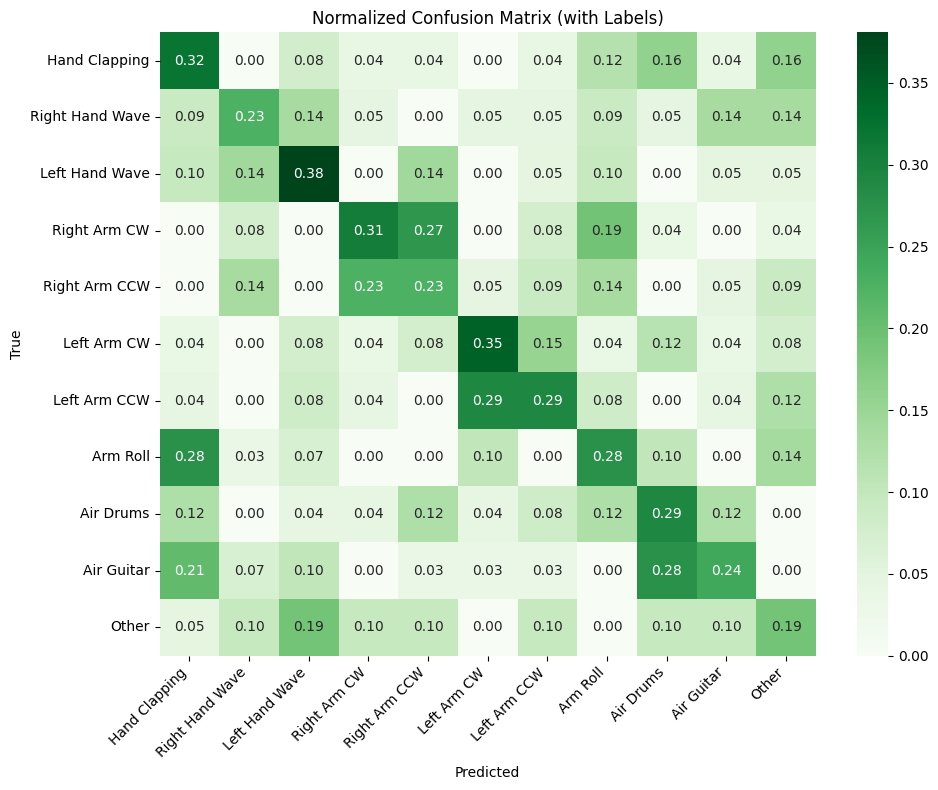
\includegraphics[width=0.55\linewidth]{Figure/STTF_Confusion_Matrix.png}
\caption{Normalized confusion matrix on DVS128 Gesture. Strongest performance on Left Hand Wave (0.38) and Left Arm CW (0.35); overlap between Arm Roll, Air Drums, and Air Guitar from similar motion patterns.}
\label{fig:STTF_Confusion_Matrix}
\end{figure}

%%%%%%%%%%%%%%%%%%%%%%%%%%%%%%%%%%%%%%%%%%%%%%%%%%%%%%%%%%%%

%\newpage
\input{checklist.tex}


\end{document}
